\documentclass{article}
\usepackage{tikz}
\usetikzlibrary{arrows.meta, positioning}

% Custom TikZ styles for cubing diagrams
\tikzset{
    cube/.style={matrix of nodes, nodes={draw, minimum size=0.6cm, anchor=center, inner sep=0pt}, column sep=-\pgflinewidth, row sep=-\pgflinewidth},
    yellowface/.style={fill=yellow!90!black},
    grayface/.style={fill=gray!40},
    pllarrow/.style={thick, -{Stealth[scale=1.2]}, red}
}

\begin{document}

\section*{One-Look OLL: Solving Orientation of Top Layer}
\centering
\section*{Fish Shapes}

% --- OLL CASE (e.g., OLL 21 / Cross "Cross") ---
% ======================== FISH SHAPES ========================
\begin{minipage}{0.45\textwidth}
\centering
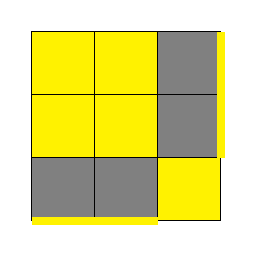
\begin{tikzpicture}[scale=0.8]
    % Draw the 3x3 Top Face Grid
    \foreach \x in {0,1,2} {
        \foreach \y in {0,1,2} {
            \draw[fill=gray] (\x,\y) rectangle (\x+1,\y+1);
        }
    }
    % Color the oriented yellow stickers on top (Fish shape representation)
    \foreach \x/\y in {2/0, 0/1, 1/1, 0/2, 1/2} {
        \draw[fill=yellow] (\x,\y) rectangle (\x+1,\y+1);
    }
    % Unoriented bars on the sides
    \draw[line width=3pt, yellow] (0,0) -- (1,0);
    \draw[line width=3pt, yellow] (1,0) -- (2,0);
    \draw[line width=3pt, yellow] (3,1) -- (3,2);
    \draw[line width=3pt, yellow] (3,2) -- (3,3);
\end{tikzpicture}

\medskip
\texttt{(F R' F' R) (U R U' R')}
\end{minipage}%
\hfill%
\begin{minipage}{0.45\textwidth}
\centering
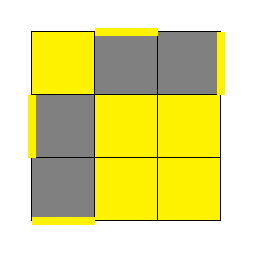
\begin{tikzpicture}[scale=0.8]
    % Draw the 3x3 Top Face Grid
    \foreach \x in {0,1,2} {
        \foreach \y in {0,1,2} {
            \draw[fill=gray] (\x,\y) rectangle (\x+1,\y+1);
        }
    }
    % Color the oriented yellow stickers on top (Fish shape representation)
    \foreach \x/\y in {1/0, 2/0, 1/1, 2/1, 0/2} {
        \draw[fill=yellow] (\x,\y) rectangle (\x+1,\y+1);
    }
    \draw[line width=3pt, yellow] (0,1) -- (0,2);
    \draw[line width=3pt, yellow] (0,0) -- (1,0);
    \draw[line width=3pt, yellow] (1,3) -- (2,3);
    \draw[line width=3pt, yellow] (3,2) -- (3,3);
\end{tikzpicture}

\medskip
\texttt{R U2 R2' (F R F' R) U2 R'}
\end{minipage}

\vspace{1cm}    % Moves onto next line

  %----------------------------------------------------%
\begin{minipage}{0.45\textwidth}
\centering
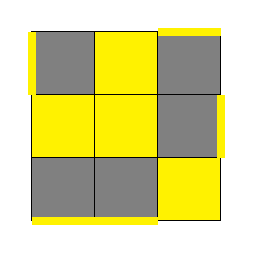
\begin{tikzpicture}[scale=0.8]
    % Draw the 3x3 Top Face Grid
    \foreach \x in {0,1,2} {
        \foreach \y in {0,1,2} {
            \draw[fill=gray] (\x,\y) rectangle (\x+1,\y+1);
        }
    }
    % Color the oriented yellow stickers on top (Fish shape representation)
    \foreach \x/\y in {2/0, 0/1, 1/1, 1/2} {
        \draw[fill=yellow] (\x,\y) rectangle (\x+1,\y+1);
    }
    % Unoriented bars on the sides
    \draw[line width=3pt, yellow] (0,2) -- (0,3);
    \draw[line width=3pt, yellow] (0,0) -- (1,0);
    \draw[line width=3pt, yellow] (1,0) -- (2,0);
    \draw[line width=3pt, yellow] (2,3) -- (3,3);
    \draw[line width=3pt, yellow] (3,1) -- (3,2);
\end{tikzpicture}

\medskip
\texttt{(R U' R' U') R' F (R2 U R' U') F'}
\end{minipage}%
\hfill%
\begin{minipage}{0.45\textwidth}
\centering
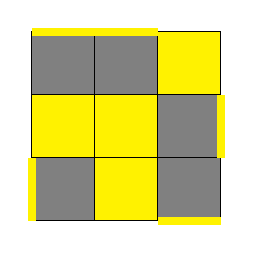
\begin{tikzpicture}[scale=0.8]
    % Draw the 3x3 Top Face Grid
    \foreach \x in {0,1,2} {
        \foreach \y in {0,1,2} {
            \draw[fill=gray] (\x,\y) rectangle (\x+1,\y+1);
        }
    }
    % Color the oriented yellow stickers on top (Fish shape representation)
    \foreach \x/\y in {1/0, 0/1, 1/1, 2,2} {
        \draw[fill=yellow] (\x,\y) rectangle (\x+1,\y+1);
    }
    \draw[line width=3pt, yellow] (0,0) -- (0,1);
    \draw[line width=3pt, yellow] (2,0) -- (3,0);
    \draw[line width=3pt, yellow] (3,1) -- (3,2);
    \draw[line width=3pt, yellow] (0,3) -- (1,3);
    \draw[line width=3pt, yellow] (1,3) -- (2,3);
\end{tikzpicture}

\medskip
\texttt{R U R' U (R' F R F') R U2 R'}
\end{minipage}

\vspace{1cm}    % Moves onto next line

% ======================== W SHAPES ========================
\section*{W Shapes}
\begin{minipage}{0.45\textwidth}
\centering
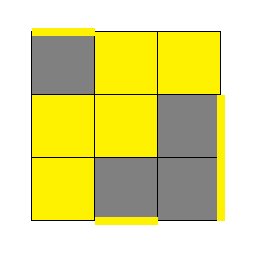
\begin{tikzpicture}[scale=0.8]
    % Draw the 3x3 Top Face Grid
    \foreach \x in {0,1,2} {
        \foreach \y in {0,1,2} {
            \draw[fill=gray] (\x,\y) rectangle (\x+1,\y+1);
        }
    }
    % Color the oriented yellow stickers on top (Fish shape representation)
    \foreach \x/\y in {0/0, 0/1, 1/1, 1/2, 2/2} {
        \draw[fill=yellow] (\x,\y) rectangle (\x+1,\y+1);
    }
    % Unoriented bars on the sides
    \draw[line width=3pt, yellow] (1,0) -- (2,0);
    \draw[line width=3pt, yellow] (3,0) -- (3,1);
    \draw[line width=3pt, yellow] (3,1) -- (3,2);
    \draw[line width=3pt, yellow] (0,3) -- (1,3);
\end{tikzpicture}

\medskip
\texttt{(R U R' U) R U' R' U' (R' F R F')}
\end{minipage}%
\hfill%
\begin{minipage}{0.45\textwidth}
\centering
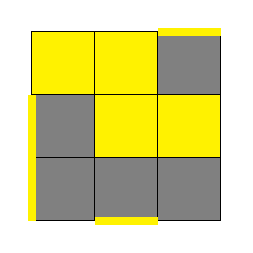
\begin{tikzpicture}[scale=0.8]
    % Draw the 3x3 Top Face Grid
    \foreach \x in {0,1,2} {
        \foreach \y in {0,1,2} {
            \draw[fill=gray] (\x,\y) rectangle (\x+1,\y+1);
        }
    }
    % Color the oriented yellow stickers on top (Fish shape representation)
    \foreach \x/\y in {0/2, 1/1, 2/1, 0/2, 1/2} {
        \draw[fill=yellow] (\x,\y) rectangle (\x+1,\y+1);
    }
    \draw[line width=3pt, yellow] (0,0) -- (0,1);
    \draw[line width=3pt, yellow] (0,1) -- (0,2);
    \draw[line width=3pt, yellow] (1,0) -- (2,0);
    \draw[line width=3pt, yellow] (2, 3) -- (3,3);
\end{tikzpicture}

\medskip
\texttt{(L' U' L U') L' U L U (r U' r' F)}
\end{minipage}

\vspace{1cm}    % Moves onto next line

% ======================== T SHAPES ========================
\section*{T Shapes}

% --- FIRST LINE: Cases 33 & 45 ---
\noindent
\begin{minipage}{0.45\textwidth}
\centering
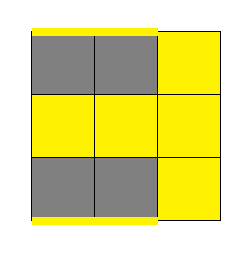
\begin{tikzpicture}[scale=0.8]
    % Draw the 3x3 Top Face Grid
    \foreach \x in {0,1,2} {
        \foreach \y in {0,1,2} {
            \draw[fill=gray] (\x,\y) rectangle (\x+1,\y+1);
        }
    }
    % Color the oriented yellow stickers on top (OLL 33)
    \foreach \x/\y in {2/0, 0/1, 1/1, 2/1, 2/2} {
        \draw[fill=yellow] (\x,\y) rectangle (\x+1,\y+1);
    }
    % Unoriented bars on the sides
    \draw[line width=3pt, yellow] (0,0) -- (1,0);
    \draw[line width=3pt, yellow] (1,0) -- (2,0);
    \draw[line width=3pt, yellow] (0,3) -- (1,3);
    \draw[line width=3pt, yellow] (1,3) -- (2,3);
\end{tikzpicture}

\medskip
\texttt{R U R' U' R' F R F'}
\end{minipage}%
\hfill%
\begin{minipage}{0.45\textwidth}
\centering
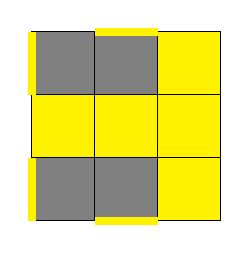
\begin{tikzpicture}[scale=0.8]
    % Draw the 3x3 Top Face Grid
    \foreach \x in {0,1,2} {
        \foreach \y in {0,1,2} {
            \draw[fill=gray] (\x,\y) rectangle (\x+1,\y+1);
        }
    }
    % Color the oriented yellow stickers on top (OLL 45)
    \foreach \x/\y in {2/0, 0/1, 1/1, 2/1, 2/2} {
        \draw[fill=yellow] (\x,\y) rectangle (\x+1,\y+1);
    }
    % Unoriented bars on the sides
    \draw[line width=3pt, yellow] (1,0) -- (2,0);
    \draw[line width=3pt, yellow] (0,0) -- (0,1);
    \draw[line width=3pt, yellow] (0,2) -- (0,3);
    \draw[line width=3pt, yellow] (1,3) -- (2,3);
\end{tikzpicture}

\medskip
\texttt{F R U R' U' F'}
\end{minipage}

\vspace{1cm}

% ======================== SQUARE SHAPE ========================
\centering
\section*{Square Shape}
% --- FIRST LINE: Cases 5 & 6 ---
\noindent
\begin{minipage}{0.45\textwidth}
\centering
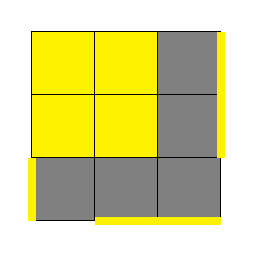
\begin{tikzpicture}[scale=0.8]
    % Draw the 3x3 Top Face Grid
    \foreach \x in {0,1,2} {
        \foreach \y in {0,1,2} {
            \draw[fill=gray] (\x,\y) rectangle (\x+1,\y+1);
        }
    }
    % Color the oriented yellow stickers on top (OLL 5)
    \foreach \x/\y in {0/1, 1/1, 0/2, 1/2} {
        \draw[fill=yellow] (\x,\y) rectangle (\x+1,\y+1);
    }
    % Unoriented bars on the sides
    \draw[line width=3pt, yellow] (0,0) -- (0,1);
    \draw[line width=3pt, yellow] (1,0) -- (2,0);
    \draw[line width=3pt, yellow] (2,0) -- (3,0);
    \draw[line width=3pt, yellow] (3,1) -- (3,2);
    \draw[line width=3pt, yellow] (3,2) -- (3,3);
\end{tikzpicture}

\medskip
\texttt{l' U2 L U L' U l}
\end{minipage}%
\hfill%
\begin{minipage}{0.45\textwidth}
\centering
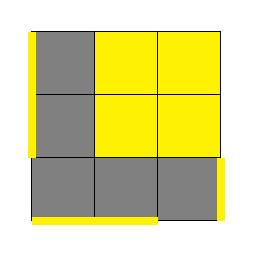
\begin{tikzpicture}[scale=0.8]
    % Draw the 3x3 Top Face Grid
    \foreach \x in {0,1,2} {
        \foreach \y in {0,1,2} {
            \draw[fill=gray] (\x,\y) rectangle (\x+1,\y+1);
        }
    }
    % Color the oriented yellow stickers on top (OLL 6)
    \foreach \x/\y in {1/1, 2/1, 1/2, 2/2} {
        \draw[fill=yellow] (\x,\y) rectangle (\x+1,\y+1);
    }
    % Unoriented bars on the sides
    \draw[line width=3pt, yellow] (0,0) -- (1,0);
    \draw[line width=3pt, yellow] (1,0) -- (2,0);
    \draw[line width=3pt, yellow] (3,0) -- (3,1);
    \draw[line width=3pt, yellow] (0,1) -- (0,2);
    \draw[line width=3pt, yellow] (0,2) -- (0,3);
\end{tikzpicture}

\medskip
\texttt{r U2 R' U' R U' r'}
\end{minipage}

\vspace{1cm}

% ======================== SMALL LIGHTNING BOLT ========================
\section*{Small Lightning Bolt}
\begin{minipage}{0.45\textwidth}
\centering
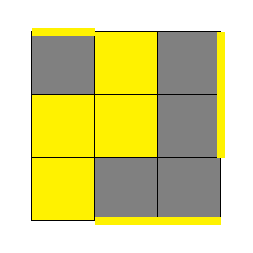
\begin{tikzpicture}[scale=0.8]
    \foreach \x in {0,1,2} { \foreach \y in {0,1,2} { \draw[fill=gray] (\x,\y) rectangle (\x+1,\y+1); } }
    % OLL 7
    \foreach \x/\y in {0/0, 0/1, 1/1, 1/2} { \draw[fill=yellow] (\x,\y) rectangle (\x+1,\y+1); }
    \draw[line width=3pt, yellow] (0,3) -- (1,3);
    \draw[line width=3pt, yellow] (1,0) -- (2,0);
    \draw[line width=3pt, yellow] (2,0) -- (3,0);
    \draw[line width=3pt, yellow] (3,1) -- (3,2);
    \draw[line width=3pt, yellow] (3,2) -- (3,3);
\end{tikzpicture}

\medskip
\texttt{r U R' U R U2 r'}
\end{minipage}%
\hfill%
\begin{minipage}{0.45\textwidth}
\centering
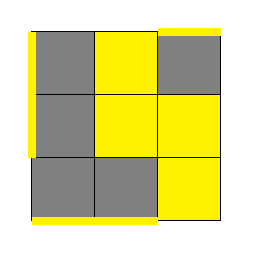
\begin{tikzpicture}[scale=0.8]
    \foreach \x in {0,1,2} { \foreach \y in {0,1,2} { \draw[fill=gray] (\x,\y) rectangle (\x+1,\y+1); } }
    % OLL 11
    \foreach \x/\y in {2/0, 1/1, 2/1, 1/2} { \draw[fill=yellow] (\x,\y) rectangle (\x+1,\y+1); }
    \draw[line width=3pt, yellow] (0,1) -- (0,2);
    \draw[line width=3pt, yellow] (0,2) -- (0,3);
    \draw[line width=3pt, yellow] (0,0) -- (1,0);
    \draw[line width=3pt, yellow] (1,0) -- (2,0);
    \draw[line width=3pt, yellow] (2,3) -- (3,3);
\end{tikzpicture}

\medskip
\texttt{r U R' U R' F R F' R U2 r'}
\end{minipage}%

\vspace{1cm}
  %-----------------------------------------------------%
\noindent
\begin{minipage}{0.45\textwidth}
\centering
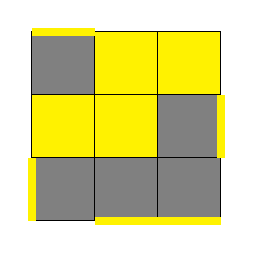
\begin{tikzpicture}[scale=0.8]
    \foreach \x in {0,1,2} { \foreach \y in {0,1,2} { \draw[fill=gray] (\x,\y) rectangle (\x+1,\y+1); } }
    % OLL 11
    \foreach \x/\y in {0/1, 1/1, 1/2, 2/2} { \draw[fill=yellow] (\x,\y) rectangle (\x+1,\y+1); }
    \draw[line width=3pt, yellow] (0,0) -- (0,1);
    \draw[line width=3pt, yellow] (0,3) -- (1,3);
    \draw[line width=3pt, yellow] (1,0) -- (2,0);
    \draw[line width=3pt, yellow] (2,0) -- (3,0);
    \draw[line width=3pt, yellow] (3,1) -- (3,2);
\end{tikzpicture}

\medskip
\texttt{r U R' U R' F R F' R U2 r'}
\end{minipage}%
\hfill%
\begin{minipage}{0.45\textwidth}
\centering
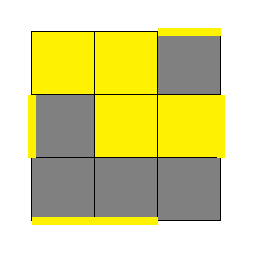
\begin{tikzpicture}[scale=0.8]
    \foreach \x in {0,1,2} { \foreach \y in {0,1,2} { \draw[fill=gray] (\x,\y) rectangle (\x+1,\y+1); } }
    % OLL 12
    \foreach \x/\y in {1/1, 2/1, 0/2, 1/2} { \draw[fill=yellow] (\x,\y) rectangle (\x+1,\y+1); }
    \draw[line width=3pt, yellow] (0,1) -- (0,2);
    \draw[line width=3pt, yellow] (0,0) -- (1,0);
    \draw[line width=3pt, yellow] (1,0) -- (2,0);
    \draw[line width=3pt, yellow] (2,3) -- (3,3);
    \draw[line width=3pt, yellow] (3,1) -- (3,2);
\end{tikzpicture}

\medskip
\texttt{M' R' U' R U' R' U2 R U' R r'}
\end{minipage}

\vspace{1cm}
% ======================== SMALL L SHAPE (Cases 47 - 54) ========================
\section*{Small L Shape}

% --- FIRST LINE: Cases 47 & 48 ---
\noindent
\begin{minipage}{0.45\textwidth}
\centering
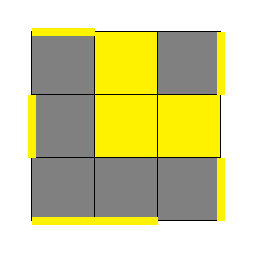
\begin{tikzpicture}[scale=0.8]
    % Draw the 3x3 Top Face Grid
    \foreach \x in {0,1,2} {
        \foreach \y in {0,1,2} {
            \draw[fill=gray] (\x,\y) rectangle (\x+1,\y+1);
        }
    }
    % Color the oriented yellow stickers on top (OLL 47)
    \foreach \x/\y in {1/1, 2/1, 1/2} {
        \draw[fill=yellow] (\x,\y) rectangle (\x+1,\y+1);
    }
    % Unoriented bars on the sides
    \draw[line width=3pt, yellow] (0,3) -- (1,3);
    \draw[line width=3pt, yellow] (0,1) -- (0,2);
    \draw[line width=3pt, yellow] (0,0) -- (1,0);
    \draw[line width=3pt, yellow] (1,0) -- (2,0);
    \draw[line width=3pt, yellow] (3,0) -- (3,1);
    \draw[line width=3pt, yellow] (3,2) -- (3,3);
\end{tikzpicture}

\medskip
\texttt{R' U' R' F R F' R' F R F' U R}
\end{minipage}%
\hfill%
\begin{minipage}{0.45\textwidth}
\centering
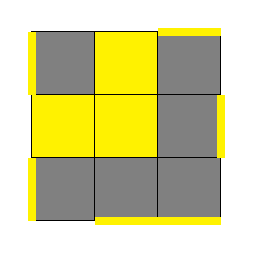
\begin{tikzpicture}[scale=0.8]
    % Draw the 3x3 Top Face Grid
    \foreach \x in {0,1,2} {
        \foreach \y in {0,1,2} {
            \draw[fill=gray] (\x,\y) rectangle (\x+1,\y+1);
        }
    }
    % Color the oriented yellow stickers on top (OLL 48)
    \foreach \x/\y in {0/1, 1/1, 1/2} {
        \draw[fill=yellow] (\x,\y) rectangle (\x+1,\y+1);
    }
    % Unoriented bars on the sides
    \draw[line width=3pt, yellow] (2,3) -- (3,3);
    \draw[line width=3pt, yellow] (0,2) -- (0,3);
    \draw[line width=3pt, yellow] (0,0) -- (0,1);
    \draw[line width=3pt, yellow] (1,0) -- (2,0);
    \draw[line width=3pt, yellow] (2,0) -- (3,0);
    \draw[line width=3pt, yellow] (3,1) -- (3,2);
\end{tikzpicture}

\medskip
\texttt{F R U R' U' R U R' U' F'}
\end{minipage}

\vspace{1cm}

% --- SECOND LINE: Cases 49 & 50 ---
\noindent
\begin{minipage}{0.45\textwidth}
\centering
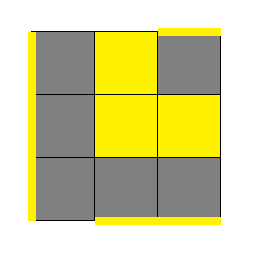
\begin{tikzpicture}[scale=0.8]
    % Draw the 3x3 Top Face Grid
    \foreach \x in {0,1,2} {
        \foreach \y in {0,1,2} {
            \draw[fill=gray] (\x,\y) rectangle (\x+1,\y+1);
        }
    }
    % Color the oriented yellow stickers on top (OLL 49)
    \foreach \x/\y in {1/1, 2/1, 1/2} {
        \draw[fill=yellow] (\x,\y) rectangle (\x+1,\y+1);
    }
    % Unoriented bars on the sides
    \draw[line width=3pt, yellow] (2,3) -- (3,3);
    \draw[line width=3pt, yellow] (0,2) -- (0,3);
    \draw[line width=3pt, yellow] (0,1) -- (0,2);
    \draw[line width=3pt, yellow] (0,0) -- (0,1);
    \draw[line width=3pt, yellow] (1,0) -- (2,0);
    \draw[line width=3pt, yellow] (2,0) -- (3,0);
\end{tikzpicture}

\medskip
\texttt{r U' r2 U r2 U r2 U' r}
\end{minipage}%
\hfill%
\begin{minipage}{0.45\textwidth}
\centering
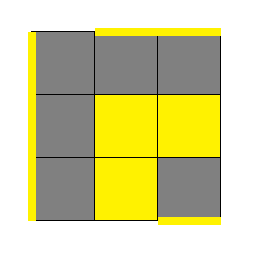
\begin{tikzpicture}[scale=0.8]
    % Draw the 3x3 Top Face Grid
    \foreach \x in {0,1,2} {
        \foreach \y in {0,1,2} {
            \draw[fill=gray] (\x,\y) rectangle (\x+1,\y+1);
        }
    }
    % Color the oriented yellow stickers on top (OLL 50)
    \foreach \x/\y in {1/0, 1/1, 2/1} {
        \draw[fill=yellow] (\x,\y) rectangle (\x+1,\y+1);
    }
    % Unoriented bars on the sides
    \draw[line width=3pt, yellow] (1,3) -- (2,3);
    \draw[line width=3pt, yellow] (2,3) -- (3,3);
    \draw[line width=3pt, yellow] (0,2) -- (0,3);
    \draw[line width=3pt, yellow] (0,1) -- (0,2);
    \draw[line width=3pt, yellow] (0,0) -- (0,1);
    \draw[line width=3pt, yellow] (2,0) -- (3,0);
\end{tikzpicture}

\medskip
\texttt{r' U r2 U' r2 U' r2 U r'}
\end{minipage}

\vspace{1cm}

% --- THIRD LINE: Cases 53 & 54 ---
\noindent
\begin{minipage}{0.45\textwidth}
\centering
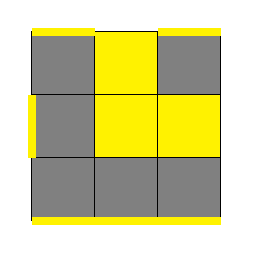
\begin{tikzpicture}[scale=0.8]
    % Draw the 3x3 Top Face Grid
    \foreach \x in {0,1,2} {
        \foreach \y in {0,1,2} {
            \draw[fill=gray] (\x,\y) rectangle (\x+1,\y+1);
        }
    }
    % Color the oriented yellow stickers on top (OLL 53)
    \foreach \x/\y in {1/1, 2/1, 1/2} {
        \draw[fill=yellow] (\x,\y) rectangle (\x+1,\y+1);
    }
    % Unoriented bars on the sides
    \draw[line width=3pt, yellow] (0,3) -- (1,3);
    \draw[line width=3pt, yellow] (2,3) -- (3,3);
    \draw[line width=3pt, yellow] (0,1) -- (0,2);
    \draw[line width=3pt, yellow] (0,0) -- (1,0);
    \draw[line width=3pt, yellow] (1,0) -- (2,0);
    \draw[line width=3pt, yellow] (2,0) -- (3,0);
\end{tikzpicture}

\medskip
\texttt{l' U2 L U L' U' L U L' U l}
\end{minipage}%
\hfill%
\begin{minipage}{0.45\textwidth}
\centering
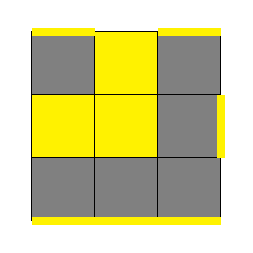
\begin{tikzpicture}[scale=0.8]
    % Draw the 3x3 Top Face Grid
    \foreach \x in {0,1,2} {
        \foreach \y in {0,1,2} {
            \draw[fill=gray] (\x,\y) rectangle (\x+1,\y+1);
        }
    }
    % Color the oriented yellow stickers on top (OLL 54)
    \foreach \x/\y in {0/1, 1/1, 1/2} {
        \draw[fill=yellow] (\x,\y) rectangle (\x+1,\y+1);
    }
    % Unoriented bars on the sides
    \draw[line width=3pt, yellow] (0,3) -- (1,3);
    \draw[line width=3pt, yellow] (2,3) -- (3,3);
    \draw[line width=3pt, yellow] (3,1) -- (3,2);
    \draw[line width=3pt, yellow] (0,0) -- (1,0);
    \draw[line width=3pt, yellow] (1,0) -- (2,0);
    \draw[line width=3pt, yellow] (2,0) -- (3,0);
\end{tikzpicture}

\medskip
\texttt{r U2 R' U' R U R' U' R U' r'}
\end{minipage}

\vspace{1cm}

% ======================== P SHAPE ========================
\section*{P Shape}

% --- FIRST LINE: Cases 31 & 32 ---
\noindent
\begin{minipage}{0.45\textwidth}
\centering
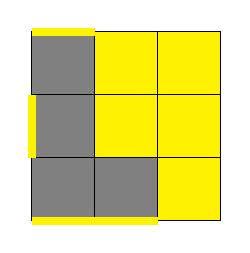
\begin{tikzpicture}[scale=0.8]
    % Draw the 3x3 Top Face Grid
    \foreach \x in {0,1,2} {
        \foreach \y in {0,1,2} {
            \draw[fill=gray] (\x,\y) rectangle (\x+1,\y+1);
        }
    }
    % Color the oriented yellow stickers on top (OLL 31)
    \foreach \x/\y in {2/0, 1/1, 2/1, 1/2, 2/2} {
        \draw[fill=yellow] (\x,\y) rectangle (\x+1,\y+1);
    }
    % Unoriented bars on the sides
    \draw[line width=3pt, yellow] (0,0) -- (1,0);
    \draw[line width=3pt, yellow] (1,0) -- (2,0);
    \draw[line width=3pt, yellow] (0,1) -- (0,2);
    \draw[line width=3pt, yellow] (0,3) -- (1,3);
\end{tikzpicture}

\medskip
\texttt{R' U' F U R U' R' F' R}
\end{minipage}%
\hfill%
\begin{minipage}{0.45\textwidth}
\centering
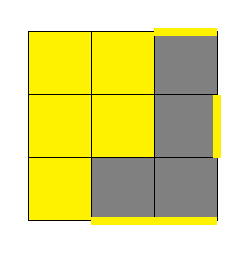
\begin{tikzpicture}[scale=0.8]
    % Draw the 3x3 Top Face Grid
    \foreach \x in {0,1,2} {
        \foreach \y in {0,1,2} {
            \draw[fill=gray] (\x,\y) rectangle (\x+1,\y+1);
        }
    }
    % Color the oriented yellow stickers on top (OLL 32)
    \foreach \x/\y in {0/0, 0/1, 1/1, 0/2, 1/2} {
        \draw[fill=yellow] (\x,\y) rectangle (\x+1,\y+1);
    }
    % Unoriented bars on the sides
    \draw[line width=3pt, yellow] (1,0) -- (2,0);
    \draw[line width=3pt, yellow] (2,0) -- (3,0);
    \draw[line width=3pt, yellow] (3,1) -- (3,2);
    \draw[line width=3pt, yellow] (2,3) -- (3,3);
\end{tikzpicture}

\medskip
\texttt{L U F' U' L' U L F L'}
\end{minipage}

\vspace{1cm}

% --- SECOND LINE: Cases 43 & 44 ---
\noindent
\begin{minipage}{0.45\textwidth}
\centering
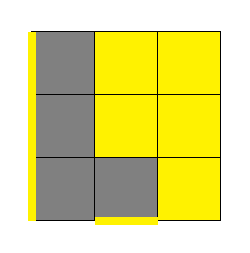
\begin{tikzpicture}[scale=0.8]
    % Draw the 3x3 Top Face Grid
    \foreach \x in {0,1,2} {
        \foreach \y in {0,1,2} {
            \draw[fill=gray] (\x,\y) rectangle (\x+1,\y+1);
        }
    }
    % Color the oriented yellow stickers on top (OLL 43)
    \foreach \x/\y in {2/0, 1/1, 2/1, 1/2, 2/2} {
        \draw[fill=yellow] (\x,\y) rectangle (\x+1,\y+1);
    }
    % Unoriented bars on the sides
    \draw[line width=3pt, yellow] (0,0) -- (0,1);
    \draw[line width=3pt, yellow] (0,1) -- (0,2);
    \draw[line width=3pt, yellow] (0,2) -- (0,3);
    \draw[line width=3pt, yellow] (1,0) -- (2,0);
\end{tikzpicture}

\medskip
\texttt{F' U' L' U L F}
\end{minipage}%
\hfill%
\begin{minipage}{0.45\textwidth}
\centering
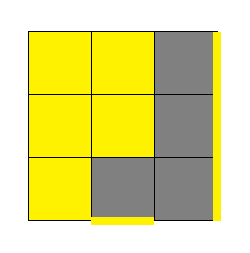
\begin{tikzpicture}[scale=0.8]
    % Draw the 3x3 Top Face Grid
    \foreach \x in {0,1,2} {
        \foreach \y in {0,1,2} {
            \draw[fill=gray] (\x,\y) rectangle (\x+1,\y+1);
        }
    }
    % Color the oriented yellow stickers on top (OLL 44)
    \foreach \x/\y in {0/0, 0/1, 1/1, 0/2, 1/2} {
        \draw[fill=yellow] (\x,\y) rectangle (\x+1,\y+1);
    }
    % Unoriented bars on the sides
    \draw[line width=3pt, yellow] (1,0) -- (2,0);
    \draw[line width=3pt, yellow] (3,0) -- (3,1);
    \draw[line width=3pt, yellow] (3,1) -- (3,2);
    \draw[line width=3pt, yellow] (3,2) -- (3,3);
\end{tikzpicture}

\medskip
\texttt{F U R U' R' F'}
\end{minipage}

\vspace{1cm}

% ======================== KNIGHT MOVE SHAPE ========================
\section*{Knight Move Shape}

% --- FIRST LINE: Cases 13 & 14 ---
\noindent
\begin{minipage}{0.45\textwidth}
\centering
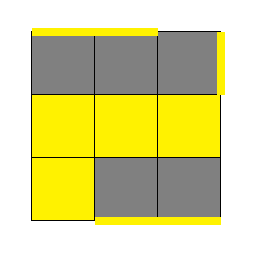
\begin{tikzpicture}[scale=0.8]
    % Draw the 3x3 Top Face Grid
    \foreach \x in {0,1,2} {
        \foreach \y in {0,1,2} {
            \draw[fill=gray] (\x,\y) rectangle (\x+1,\y+1);
        }
    }
    % Color the oriented yellow stickers on top (OLL 13)
    \foreach \x/\y in {0/0, 0/1, 1/1, 2/1} {
        \draw[fill=yellow] (\x,\y) rectangle (\x+1,\y+1);
    }
    % Unoriented bars on the sides
    \draw[line width=3pt, yellow] (1,0) -- (2,0);
    \draw[line width=3pt, yellow] (2,0) -- (3,0);
    \draw[line width=3pt, yellow] (0,3) -- (1,3);
    \draw[line width=3pt, yellow] (1,3) -- (2,3);
    \draw[line width=3pt, yellow] (3,2) -- (3,3);
\end{tikzpicture}

\medskip
\texttt{F U R U' R2 F' R U R U' R'}
\end{minipage}%
\hfill%
\begin{minipage}{0.45\textwidth}
\centering
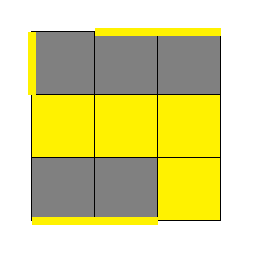
\begin{tikzpicture}[scale=0.8]
    % Draw the 3x3 Top Face Grid
    \foreach \x in {0,1,2} {
        \foreach \y in {0,1,2} {
            \draw[fill=gray] (\x,\y) rectangle (\x+1,\y+1);
        }
    }
    % Color the oriented yellow stickers on top (OLL 14)
    \foreach \x/\y in {2/0, 0/1, 1/1, 2/1} {
        \draw[fill=yellow] (\x,\y) rectangle (\x+1,\y+1);
    }
    % Unoriented bars on the sides
    \draw[line width=3pt, yellow] (0,0) -- (1,0);
    \draw[line width=3pt, yellow] (1,0) -- (2,0);
    \draw[line width=3pt, yellow] (0,2) -- (0,3);
    \draw[line width=3pt, yellow] (1,3) -- (2,3);
    \draw[line width=3pt, yellow] (2,3) -- (3,3);
\end{tikzpicture}

\medskip
\texttt{R' F R U R' F' R F U' F'}
\end{minipage}

\vspace{1cm}

  % --------------------------------------------%
\noindent
\begin{minipage}{0.45\textwidth}
\centering
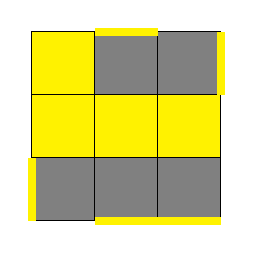
\begin{tikzpicture}[scale=0.8]
    % Draw the 3x3 Top Face Grid
    \foreach \x in {0,1,2} {
        \foreach \y in {0,1,2} {
            \draw[fill=gray] (\x,\y) rectangle (\x+1,\y+1);
        }
    }
    % Color the oriented yellow stickers on top (OLL 15)
    \foreach \x/\y in {0/1, 1/1, 2/1, 0/2} {
        \draw[fill=yellow] (\x,\y) rectangle (\x+1,\y+1);
    }
    % Unoriented bars on the sides
    \draw[line width=3pt, yellow] (1,3) -- (2,3);
    \draw[line width=3pt, yellow] (3,2) -- (3,3);
    \draw[line width=3pt, yellow] (0,0) -- (0,1);
    \draw[line width=3pt, yellow] (1,0) -- (2,0);
    \draw[line width=3pt, yellow] (2,0) -- (3,0);
\end{tikzpicture}

\medskip
\texttt{l' U' l L' U' L U l' U l}
\end{minipage}%
\hfill%
\begin{minipage}{0.45\textwidth}
\centering
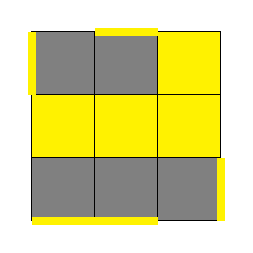
\begin{tikzpicture}[scale=0.8]
    % Draw the 3x3 Top Face Grid
    \foreach \x in {0,1,2} {
        \foreach \y in {0,1,2} {
            \draw[fill=gray] (\x,\y) rectangle (\x+1,\y+1);
        }
    }
    % Color the oriented yellow stickers on top (OLL 16)
    \foreach \x/\y in {0/1, 1/1, 2/1, 2/2} {
        \draw[fill=yellow] (\x,\y) rectangle (\x+1,\y+1);
    }
    % Unoriented bars on the sides
    \draw[line width=3pt, yellow] (1,3) -- (2,3);
    \draw[line width=3pt, yellow] (0,2) -- (0,3);
    \draw[line width=3pt, yellow] (3,0) -- (3,1);
    \draw[line width=3pt, yellow] (0,0) -- (1,0);
    \draw[line width=3pt, yellow] (1,0) -- (2,0);
\end{tikzpicture}

\medskip
\texttt{r U r' R U R' U' r U' r'}
\end{minipage}

\vspace{1cm}

% ======================== I SHAPE ========================
\section*{I Shape}

% --- FIRST LINE: Cases 51 & 52 ---
\noindent
\begin{minipage}{0.45\textwidth}
\centering
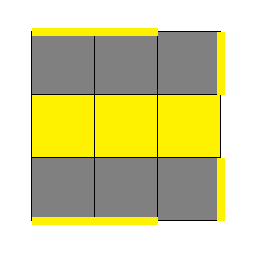
\begin{tikzpicture}[scale=0.8]
    \foreach \x in {0,1,2} { \foreach \y in {0,1,2} { \draw[fill=gray] (\x,\y) rectangle (\x+1,\y+1); } }
    % OLL 51 rotated 180
    \foreach \x/\y in {0/1, 1/1, 2/1} { \draw[fill=yellow] (\x,\y) rectangle (\x+1,\y+1); }
    \draw[line width=3pt, yellow] (3,2) -- (3,3);
    \draw[line width=3pt, yellow] (3,0) -- (3,1);
    \draw[line width=3pt, yellow] (1,3) -- (2,3);
    \draw[line width=3pt, yellow] (0,3) -- (1,3);
    \draw[line width=3pt, yellow] (1,0) -- (2,0);
    \draw[line width=3pt, yellow] (0,0) -- (1,0);
\end{tikzpicture}

\medskip
\texttt{F U R U' R' U R U' R' F'}
\end{minipage}%
\hfill%
\begin{minipage}{0.45\textwidth}
\centering
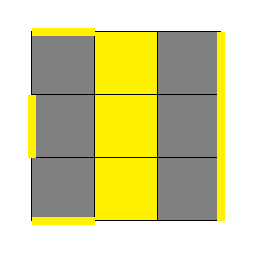
\begin{tikzpicture}[scale=0.8]
    \foreach \x in {0,1,2} { \foreach \y in {0,1,2} { \draw[fill=gray] (\x,\y) rectangle (\x+1,\y+1); } }
    % OLL 52 rotated 180 (horizontal bar)
    \foreach \x/\y in {1/0, 1/1, 1/2} { \draw[fill=yellow] (\x,\y) rectangle (\x+1,\y+1); }
    \draw[line width=3pt, yellow] (0,1) -- (0,2);
    \draw[line width=3pt, yellow] (0,0) -- (1,0);
    \draw[line width=3pt, yellow] (0,3) -- (1,3);
    \draw[line width=3pt, yellow] (3,0) -- (3,1);
    \draw[line width=3pt, yellow] (3,1) -- (3,2);
    \draw[line width=3pt, yellow] (3,2) -- (3,3);
\end{tikzpicture}

\medskip
\texttt{R U R' U R U' B U' B' R'}
\end{minipage}

\vspace{1cm}

% --- SECOND LINE: Cases 55 & 56 ---
\noindent
\begin{minipage}{0.45\textwidth}
\centering
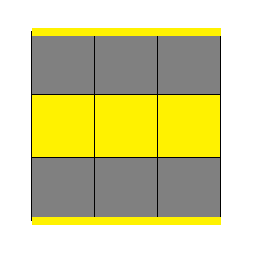
\begin{tikzpicture}[scale=0.8]
    % Draw the 3x3 Top Face Grid
    \foreach \x in {0,1,2} {
        \foreach \y in {0,1,2} {
            \draw[fill=gray] (\x,\y) rectangle (\x+1,\y+1);
        }
    }
    % Oriented yellow stickers on top: Horizontal "I" bar
    \foreach \x/\y in {0/1, 1/1, 2/1} {
        \draw[fill=yellow] (\x,\y) rectangle (\x+1,\y+1);
    }
    % Unoriented bars on the sides
    \draw[line width=3pt, yellow] (0,0) -- (1,0);
    \draw[line width=3pt, yellow] (1,0) -- (2,0);
    \draw[line width=3pt, yellow] (2,0) -- (3,0);
    \draw[line width=3pt, yellow] (0,3) -- (1,3);
    \draw[line width=3pt, yellow] (1,3) -- (2,3);
    \draw[line width=3pt, yellow] (2,3) -- (3,3);
\end{tikzpicture}

\medskip
\texttt{R' F R U R U' R2 F' R2 U' R' U R U R'}
\end{minipage}
\hfill%
\begin{minipage}{0.45\textwidth}
\centering
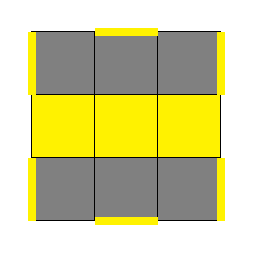
\begin{tikzpicture}[scale=0.8]
    % Draw the 3x3 Top Face Grid
    \foreach \x in {0,1,2} {
        \foreach \y in {0,1,2} {
            \draw[fill=gray] (\x,\y) rectangle (\x+1,\y+1);
        }
    }
    % Color the oriented yellow stickers on top (OLL 56)
    \foreach \x/\y in {0/1, 1/1, 2/1} {
        \draw[fill=yellow] (\x,\y) rectangle (\x+1,\y+1);
    }
    % Unoriented bars on the sides
    \draw[line width=3pt, yellow] (0,0) -- (0,1);
    \draw[line width=3pt, yellow] (0,2) -- (0,3);
    \draw[line width=3pt, yellow] (3,0) -- (3,1);
    \draw[line width=3pt, yellow] (3,2) -- (3,3);
    \draw[line width=3pt, yellow] (1,0) -- (2,0);
    \draw[line width=3pt, yellow] (1,3) -- (2,3);
\end{tikzpicture}

\medskip
\texttt{r' U' r U' R' U R U' R' U R r' U r}
\end{minipage}
\end{document}